\documentclass[dvipsnames,border=3pt]{standalone}
\usepackage{tikz}
\usetikzlibrary{arrows}
\usetikzlibrary{shapes}
\usepackage{enumitem}
\usepackage{bm}
\usepackage{mathdots}
\usepackage{amsmath}
\usetikzlibrary{shadings}
\usetikzlibrary{decorations.pathreplacing}
\usepackage{helvet}
\usetikzlibrary{arrows.meta}
\usepackage{graphicx}
\usepackage{pgfplots}
\usepackage{pgfplotstable}
\usepackage{filecontents}
\usetikzlibrary{plotmarks}
\usetikzlibrary{shapes.misc}
\pgfplotsset{compat=newest}

\renewcommand{\familydefault}{\sfdefault}

\definecolor{mylightgray}{cmyk}{0,0,0,0.1}
\usetikzlibrary{arrows,decorations.pathmorphing,backgrounds,fit,positioning,shapes.symbols,chains}

\begin{document}

\begin{tikzpicture}
    % trim=left botm right top
    
    \node at (4.5,2.4) {\LARGE \textbf{Mixed effects data: interactions and main effects}};
    
    \draw[-latex, line width=1mm,draw=gray!70] (3.62,0) -- (5.23,0);
    
    \draw[-latex, line width=1mm,draw=gray!70] (9,-1.76) -- (9,-2.67);

    \draw[-latex, line width=1mm,draw=gray!70] (1.37,-5.3) -- (-0.23,-5.3);
    
    \draw[-latex,line width=1mm,draw=gray!70] (-3,-6.55) -- (-3,-9.55);
    
    \draw[-latex,line width=1mm,draw=gray!70] (0.8,-11.42) -- (1.67,-11.42);
    
    \draw[-latex,line width=1mm,draw=gray!70] (7.15,-11.42) -- (6.29,-11.42);
    
    \node at (0,0) (1) {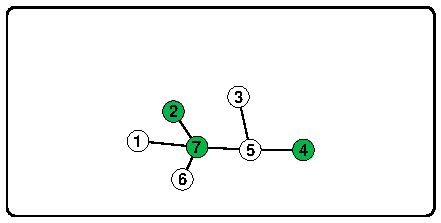
\includegraphics[clip,trim=0.1cm 0.1cm 0.1cm 0.1cm]{interaction_simulation1.pdf}};
    
    \node at (9,0) (2) {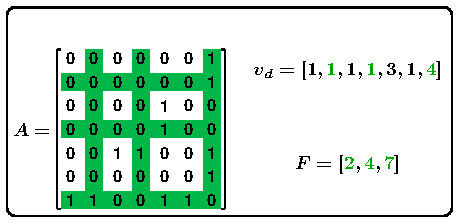
\includegraphics[clip,trim=0.1cm 0.1cm 0.1cm 0.1cm]{interaction_simulation2.pdf}};
    
    \node at (8.5,-5.3) (3) {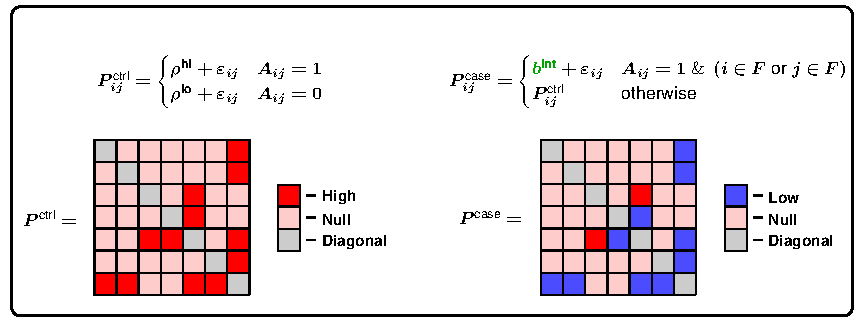
\includegraphics[clip,trim=0.1cm 0.1cm 0.1cm 0.1cm]{interaction_simulation3.pdf}};
    
    \node at (-3,-5.3) (4) {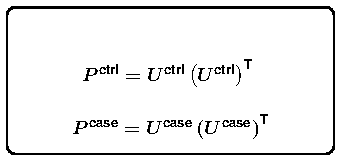
\includegraphics[clip,trim=0.1cm 0.1cm 0.1cm 0.1cm]{interaction_simulation4.pdf}};
    
    \node at (-2.5,-11.42) (5) {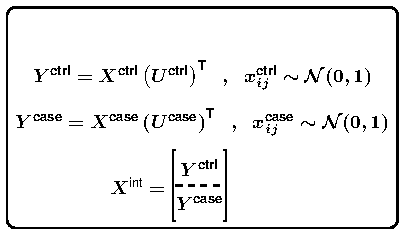
\includegraphics[clip,trim=0.1cm 0.1cm 0.1cm 0.1cm]{interaction_simulation5.pdf}};
    
    \node at (11.45,-11.42) (6) {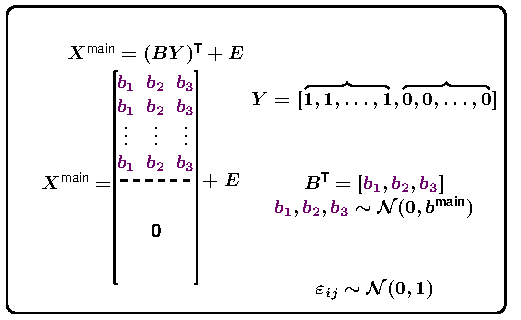
\includegraphics[clip,trim=0.1cm 0.1cm 0.1cm 0.1cm]{main_effect_added_to_interaction.pdf}};
    
    \node at (3.98,-11.12) (7) {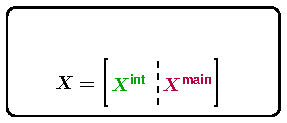
\includegraphics[clip,trim=0.1cm 0.1cm 0.1cm 0.1cm]{mixed_effects_combining_main-interaction.pdf}};
    
    %%%%%%%%%%%%%%%%%%%%%%%%%%%%%%%%%%%%%%% box 1 %%%%%%%%%%%%%%%%%%%%%%%%%%%%%%%%%%%%%%%%%%%%%%%
    \node[circle,draw,line width=0.2mm,xscale=1.4,yscale=1.4,fill=gray!40] at (-3.3,1.45) {};
    \node at (-3.3,1.45) {\textbf{1}};
    
    \node[xscale=1,yscale=1] at (0,0.9) {\textbf{Erd\H{o}s-R\'{e}nyi or Scale-free}};
    %\node[xscale=1,yscale=1] at (2.28,0.9) {\textbf{Erdos-Renyi}};
    %\node[xscale=1,yscale=1] at (0,0.9) {\textbf{or}};
    \node[xscale=1,yscale=1] at (0,1.45) {\textbf{Random graph}};
    %%%%%%%%%%%%%%%%%%%%%%%%%%%%%%%%%%%%%%% box 1 %%%%%%%%%%%%%%%%%%%%%%%%%%%%%%%%%%%%%%%%%%%%%%%
    
    %%%%%%%%%%%%%%%%%%%%%%%%%%%%%%%%%%%%%%% box 2 %%%%%%%%%%%%%%%%%%%%%%%%%%%%%%%%%%%%%%%%%%%%%%%
    \node[circle,draw,line width=0.2mm,xscale=1.4,yscale=1.4,fill=gray!40] at (5.55,1.45) {};
    \node at (5.55,1.45) {\textbf{2}};
    
    \node[xscale=1,yscale=1] at (7.5,1.45) {\textbf{Adjacency matrix}};
    \node[xscale=1,yscale=1] at (11,1.2) {\textbf{Degree vector}};
    \node[xscale=1,yscale=1] at (11,-0.4) {\textbf{Functional features}};
    %%%%%%%%%%%%%%%%%%%%%%%%%%%%%%%%%%%%%%% box 2 %%%%%%%%%%%%%%%%%%%%%%%%%%%%%%%%%%%%%%%%%%%%%%%
    
    %%%%%%%%%%%%%%%%%%%%%%%%%%%%%%%%%%%%%%% box 3 %%%%%%%%%%%%%%%%%%%%%%%%%%%%%%%%%%%%%%%%%%%%%%%
    \node[circle,draw,line width=0.2mm,xscale=1.4,yscale=1.4,fill=gray!40] at (1.7,-3.01) {};
    \node at (1.7,-3.01) {\textbf{3}};
    
    \node[xscale=1,yscale=1] at (8.5,-2.94) {\textbf{Correlation matrices}};
    
    \node[xscale=1,yscale=1] at (4.1,-4.7) {\textbf{Controls}};
    \node[xscale=1,yscale=1] at (11.65,-4.7) {\textbf{Cases}};
    %%%%%%%%%%%%%%%%%%%%%%%%%%%%%%%%%%%%%%% box 3 %%%%%%%%%%%%%%%%%%%%%%%%%%%%%%%%%%%%%%%%%%%%%%%
    
    %%%%%%%%%%%%%%%%%%%%%%%%%%%%%%%%%%%%%%% box 4 %%%%%%%%%%%%%%%%%%%%%%%%%%%%%%%%%%%%%%%%%%%%%%%
    \node[circle,draw,line width=0.2mm,xscale=1.4,yscale=1.4,fill=gray!40] at (-5.45,-4.37) {};
    \node at (-5.45,-4.37) {\textbf{4}};
    \node[xscale=1,yscale=1] at (-2.7,-4.35) {\textbf{Cholesky decomposition}};
    %%%%%%%%%%%%%%%%%%%%%%%%%%%%%%%%%%%%%%% box 4 %%%%%%%%%%%%%%%%%%%%%%%%%%%%%%%%%%%%%%%%%%%%%%%
    
    %%%%%%%%%%%%%%%%%%%%%%%%%%%%%%%%%%%%%%% box 5 %%%%%%%%%%%%%%%%%%%%%%%%%%%%%%%%%%%%%%%%%%%%%%%
    \node[circle,draw,line width=0.2mm,xscale=1.4,yscale=1.4,fill=gray!40] at (-5.49,-9.87) {};
    \node at (-5.49,-9.87) {\textbf{5}};
    \node[xscale=1,yscale=1] at (-2.5,-9.85) {\textbf{Interaction data}};
    %%%%%%%%%%%%%%%%%%%%%%%%%%%%%%%%%%%%%%% box 5 %%%%%%%%%%%%%%%%%%%%%%%%%%%%%%%%%%%%%%%%%%%%%%%
    
    %%%%%%%%%%%%%%%%%%%%%%%%%%%%%%%%%%%%%%% box 6 %%%%%%%%%%%%%%%%%%%%%%%%%%%%%%%%%%%%%%%%%%%%%%%
    \node[circle,draw,line width=0.2mm,xscale=1.4,yscale=1.4,fill=gray!40] at (7.47,-9.14) {};
    \node at (7.47,-9.14) {\textbf{6}};
    \node[xscale=1,yscale=1] at (9.7,-9.14) {\textbf{Design matrix}};
    
    \node[xscale=1,yscale=1] at (13.35,-9.4) {\textbf{Binary outcome}};
    
    \node[xscale=1,yscale=1] at (12.87,-9.9) {\textbf{Cases}};
    \node[xscale=1,yscale=1] at (14.57,-9.9) {\textbf{Controls}};
    
    \node[xscale=1,yscale=1] at (13.35,-11.3) {\textbf{Effect sizes}};
    
    \node[xscale=1,yscale=1] at (13.35,-13.1) {\textbf{Gaussian noise}};
    %%%%%%%%%%%%%%%%%%%%%%%%%%%%%%%%%%%%%%% box 6 %%%%%%%%%%%%%%%%%%%%%%%%%%%%%%%%%%%%%%%%%%%%%%%
    
    %%%%%%%%%%%%%%%%%%%%%%%%%%%%%%%%%%%%%%% box 7 %%%%%%%%%%%%%%%%%%%%%%%%%%%%%%%%%%%%%%%%%%%%%%%
    \node[circle,draw,line width=0.2mm,xscale=1.4,yscale=1.4,fill=gray!40] at (2,-10.53) {};
    \node at (2,-10.53) {\textbf{7}};
    \node[xscale=1,yscale=1] at (4.2,-10.53) {\textbf{Mixed effects data}};
    %%%%%%%%%%%%%%%%%%%%%%%%%%%%%%%%%%%%%%% box 7 %%%%%%%%%%%%%%%%%%%%%%%%%%%%%%%%%%%%%%%%%%%%%%%
    
\end{tikzpicture}
    
\end{document}